\documentclass[a4paper, 10pt, twocolumn, twoside]{article}

\usepackage{ISARC}

\usepackage{lscape}
\usepackage{hologo}
\usepackage{multirow}

\begin{document}

 % Do not change the following line
\linespread{0.5}

\title{BIM-FM interoperability: integrating existing FM platform with visualization of IFC models}

\author{Andressa Oliveira$^{1}$, José Granja$^1$, Pedro Machado$^2$, Ali Motamedi$^3$, and Miguel Azenha$^1$}

\affiliation{
$^1$University of Minho, ISISE, ARISE, Department of Civil Engineering, Portugal\\
$^2$Matosinhos City Council, Portugal\\
$^2$Université du Québec à Montreal, École de Technologie Supérieure, Canada
}

\email{
\href{mailto:soliveira.andressa@gmail.com}{Email Andressa Oliveira}, 
\href{mailto:granja@civil.uminho.pt}{Email José Granja},
\href{mailto:pedro.machado@cm-matosinhos.pt}{Email Pedro Machado},
\href{mailto:ali.motamedi@etsmtl.ca}{Email Ali Motamedi},
\href{mailto:miguel.azenha@gmail.com}{Email Miguel Azenha}
}


% Do not change the following three lines
\maketitle 
\thispagestyle{fancy} 
\pagestyle{fancy}

\begin{abstract}
This article documents the developments from a collaboration with the Matosinhos City Hall in Portugal. The collaboration included the development of a web platform to integrate a management software already in use by the city hall, with 3D visualization capabilities, and the development of information requirements to guide the preparation of information models to be visualized on the platform. The platform enables the visualization of 3D models developed according to the IFC (Industry Foundation Classes) schema using the IFCjs library to manipulate, investigate and visualize IFC files. In addition, the web platform enables access to and manipulation of operational data through the 3D model. The framework presented in this paper demonstrates how the IFC model elements are linked to the Infraspeak database. This solution addresses current operational limitations and promotes broader BIM adoption in the FM sector.
\end{abstract}

\begin{keywords}
Facility Management (FM); Building Information Modelling (BIM); Interoperability; Integration; Web Platform
\end{keywords}

% AS SESSÕES DO ARTIGO COMEÇAM AQUI

\section{Introduction}
\label{sec:Introduction}

Facility Management (FM) plays a critical role in ensuring facilities' functionality, comfort, and safety \cite{IFMA2023}. The adoption of Building Information Modelling (BIM) by facility managers to enhance operational efficiency introduces unique challenges \cite{Pinti2022}. To promote a broader implementation of BIM in FM, it is essential to advance professional knowledge of information management processes that align with ISO 19650 series guidelines and have computational resources to support such digitalization. While computerized management platforms are widely utilized, the effectiveness of these systems depends on their ability to integrate diverse data sources \cite{Durdyev2022, Siccardi2023}. This includes incorporating three-dimensional models to enable comprehensive and efficient management. Within this context, a collaboration between Matosinhos City Hall (CMMatosinhos) in Portugal and the University of Minho (UMinho) aimed to enhance municipal asset management by integrating BIM methodology into the Intelligent Maintenance Management Platform (IMMP) already employed by CMMatosinhos (Infraspeak). Currentlly the IMMP provides access to a web interface that lacks the capacity for visualizing buildings and assets.

\section{Development methodology and functional requirements identification}
\label{sec:methodology}

The collaboration aimed to develop a web platform that integrates CMMatosinhos's IMMP and allows 3D visualization of buildings, enabling users to consult, edit, and add information about the assets. It involved defining information requirements for models to be used on this platform. The foreseen platform's functionalities included a building selection interface, comprehensive 3D visualization of buildings and elements, displaying building and assets identification and open requests, and enabling managers to access the IMMP page for details. Users can also submit requests for specific assets. Two main pages have been identified for the web platform: the building selection page and the interaction page, supporting two user profiles: manager and common user. Both can visualize the building in 3D, view identification information, and submit requests. Managers can also access open requests and IMMP pages. The frontend uses HTML, CSS, and JavaScript, with the IFCjs library for the interactive viewer and investigation of the IFC file. The backend is built in Python with the Flask framework. The building was modelled using Autodesk Revit 2023 and exported in the IFC4 ADD2 TC1 schema, following the information requirements developed for this research (section \ref{subsec:loin}).

\section{Implementation}
\label{sec:implementation}

To develop the proposed solution, the 'IMMP database' must be integrated into a web platform presenting the IFC model visualization. This integration necessitates the web platform to establish a correlation between specific assets within the IFC model and their equivalent within the IMMP platform. Achieving this integration depends on the unique identification of elements across both data sources and establishing a mapping between them. For the mapping, it is essential to comprehend how the assets are identified within the IMMP database (IMMP identifiers) and how CMMatosinhos identifies them in its inventory (CMMatosinhos identifiers). The 'CMMatosinhos identifiers' will be organized as part of the alphanumeric information requirements for the model (as detailed in section \ref{subsec:loin}). These identifiers will become properties associated with various elements within the model, correlating them to corresponding items in the CMMatosinhos inventory. In contrast, the 'IMMP identifiers' will not be included in the IFC model but will be used to establish a one-to-one mapping between the elements in the IMMP database and those in the model.

\subsection{Unique identifiers}
\label{subsec:identifiers}

Considering the functionalities to be implemented (section \ref{sec:methodology}), three types of elements are essential: \emph{locations}, \emph{equipment} and \emph{requests}. \emph{Locations} represent spatial assets that comprise the buildings and are essential to the equipment's localization. \emph{Equipment} is any physical asset from the CMMatosinhos' inventory (vehicles, chairs, ladders, etc.). Finally, \emph{requests} represent the solicitation for an operation action to be carried out and are always associated with the other types of elements (\emph{equipment} or \emph{location}).

\paragraph{IMMP identifier}: The IMMP database contains two categories for entering elements of the type \emph{location}: LOCATION and ELEMENT. Within the LOCATION category, \emph{locations} are organized hierarchically (from buildings to zones and to rooms) and identified by the attribute 'local\_id'. Within the second category (ELEMENT), it is possible to enter elements of two types: EQUIPMENT and LOCAL. Therefore, the \emph{locations} classified as ELEMENT are of the type LOCAL and represent only individual rooms (i.e. an office but never a building). Regarding the elements of type \emph{equipment}, those are entries of the ELEMENT category and EQUIPMENT type, and the 'element\_id' attribute uniquely identifies each element. Therefore, the 'local\_id' and 'element\_id' attributes are the IMMP identifiers for \emph{locations} and \emph{equipment}. For the \emph{requests} elements, those designated as 'open' are relevant for this work since they still require actions. Each open \emph{request} is uniquely identified by the 'failure\_id' attribute and includes a 'local\_id' attribute that specifies the \emph{location} associated with the \emph{request}. Contrarily, information regarding its connection to \emph{equipment} is accessed through the relationships of the \emph{equipment} elements, which contain the corresponding 'failure\_id' codes. The 'IMMP identifiers' established here are generated automatically by the IMMP, being a sequence of numbers (e.g. 586188) that do not correspond to the CMMatosinhos inventory.

\paragraph{CMMatosinhos identifier}: 'CMMatosinhos identifiers' refers to the coding used by CMMatosinhos to identify its assets within its inventory. Each asset within the IMMP has a unique identifier specific to the IMMP (explained previously) but also includes the CMMatosinhos inventory code associated with one of its attributes. From the three elements (\emph{equipment}, \emph{location}, and \emph{requests}), \emph{requests} do not have a CMMatosinhos identifier as they do not represent physical assets, being not part of CMMatosinhos' inventory. As for \emph{locations}, the value of the 'full\_code' attribute represents the codification used by CMMatosinhos to identify spaces, and it contains a unique code for each location (e.g. 009.G1.P0.048). For \emph{equipment}, the value of the 'code' attribute is a potential unique identifier. Within the CMMatosinhos inventory, the value of this attribute relates to the type of equipment (e.g. \#CAD.ESCR.0056 for an office chair). However, considering that there are cases where multiple \emph{equipment} share the same inventory code, a combination of the 'code' attribute of the equipment and the 'full\_code' attribute of the location where it is situated has been defined for identifying elements within the equipment group.

\subsection{Level of information need}
\label{subsec:loin}

The information requirements developed in this work include the level of information need \cite{17412-1}. Given the platform features (section \ref{sec:methodology}), the purpose for the model is the visualization of the building and assets, incorporating only alphanumerical information for building identificaton and integration with the IMMP. Table \ref{tab_loin_building} presents the level of information need for the building as a whole, where Code represents the 'CMMatosinhos identifier'.

\begin{table}[!htb]
    \renewcommand{\arraystretch}{2}
    \centering
    \caption{Level of information need for the building}
    \label{tab_loin_building}
    \begin{tabular}{l|l|l}
    \hline
    {l}\textbf{Objects:} & \multicolumn{2}{l}{\textbf{Building}}\\
    \hline
    {l}\textbf{IFC Class:} & \multicolumn{2}{l}{\textbf{IfcBuilding}}\\
    \hline
    \multicolumn{3}{l}{\textbf{Alphanumerical information}} \\
    \hline
    \multicolumn{3}{l}{Attributes} \\
    \hline
    & Attribute name & Content\\
    \hline
    & LongName & Name\\
    \hline
    \multicolumn{3}{l}{Properties} \\
    \hline
    Group & Property name & Content\\
    \hline
    ** & Local\_CMMatosinhos & Code\\
    \hline
    \textbf{Legend} & \multicolumn{2}{l}{\textbf{**}}\\
    & \multicolumn{2}{l}{CMMatosinhos\_Identification}\\
    \hline
    \end{tabular}
\end{table}

Regarding the elements composing the building and its interior, out of the three defined element types (\emph{locations}, \emph{equipment}, and \emph{requests}), \emph{requests} were excluded as their visualization is not necessary. Three main groups were established for modelling: architectural elements, equipment, and locations (table \ref{tab_loin_equipment}). Architectural elements serve for visualization and only require geometrical information. The alphanumerical information required for locations and equipment relates to the 'CMMatosinhos identifiers' and also some additional information for identifying and classifying the assets.

\begin{table*}[!htb]
    \renewcommand{\arraystretch}{1.4}
    \centering
    \caption{Level of information need for architectural elements, equipment and locations}
    \label{tab_loin_equipment}
    \begin{tabular}{p{0.8cm}|p{3.7cm}|p{3.2cm}p{3.2cm}p{2.0cm}}
    \hline
    \multicolumn{2}{l}{\textbf{Objects:}} & \textbf{Archit. elements} & \textbf{Equipment} & \textbf{Locations}\\
    \hline
    \multicolumn{2}{l}{\textbf{IFC Class:}} & \textbf{Variable} & \textbf{Variable} & \textbf{IfcSpace}\\
    \hline
    \multicolumn{5}{l}{\textbf{Geometrical information}} \\
    \hline
    \multicolumn{2}{l}{Detail} & Real representation of external limits. Single element without layers or components. & Simplified outer shell, real volumes and dimensions. Single element without layers or components. & Real volume.\\
    \multicolumn{2}{l}{Dimensionality} & 3D & 3D & 3D\\
    \multicolumn{2}{l}{Location} & Relative & Relative & Relative\\
    \multicolumn{2}{l}{Appearance} & Colour must be similar to reality, without textures. & Colour must be similar to reality, without textures. & Not visible\\
    \hline
    \multicolumn{5}{l}{\textbf{Alphanumerical information}} \\
    \hline
    \multicolumn{5}{l}{Attributes} \\
    \hline
    & Attribute name & \multicolumn{3}{c}{Content}\\
    \hline
    & LongName & X & X & Name\\
    \hline
    \multicolumn{5}{l}{Properties} \\
    \hline
    Group & Property name & \multicolumn{3}{c}{Content}\\
    \hline
    \multirow{4}{*}{**} & Codigo\_CMMatosinhos & X & Code & X\\
    & Local\_CMMatosinhos & X & X & Code\\
    & Categoria\_CMMatosinhos & X & Category & X\\
    & Tipo\_CMMatosinhos & X & Category description & X\\
    \hline
   \multirow{6}{*}{\rotatebox{90}{\textbf{Legend}}} & \multicolumn{4}{l}{\textbf{Variable}}\\
    & \multicolumn{4}{l}{    IFC classes vary depending on the architectural element or equipment.}\\
    & \multicolumn{4}{l}{\textbf{**}}\\
    & \multicolumn{4}{l}{    Name of group of properties: CMMatosinhos\_Identification}\\
    & \multicolumn{4}{l}{\textbf{X}}\\
    & \multicolumn{4}{l}{    Objects of this type must not contain this property or attribute.}\\
    \hline
    \end{tabular}
\end{table*}

\subsection{Web platform}
\label{subsec:platform}

Figure \ref{fig_fluxo} shows the information flow between the platform's frontend and backend and how the platform reacts to the manager's interactions. When a manager selects a building from a dropdown, a request retrieves the IFC file from the models' database and information from the IMMP database. Following, a 3D visualization of the building is displayed for the user, while the IFC file is investigated to retrieve the 'CMMatosinhos identifiers' of the building elements. The backend combines these 'CMMatosinhos identifiers' with 'IMMP identifiers' to map elements from both sources. This mapping allows for the identification of elements with open requests, enabling the visualization to filter and display only those elements. Additionally, the number of open requests related to the building is counted and presented to the user. Following this, users can interact with the model, view detailed asset information, access the asset's IMMP page, or create linked requests.

\begin{figure}[!htb]
    \centering
    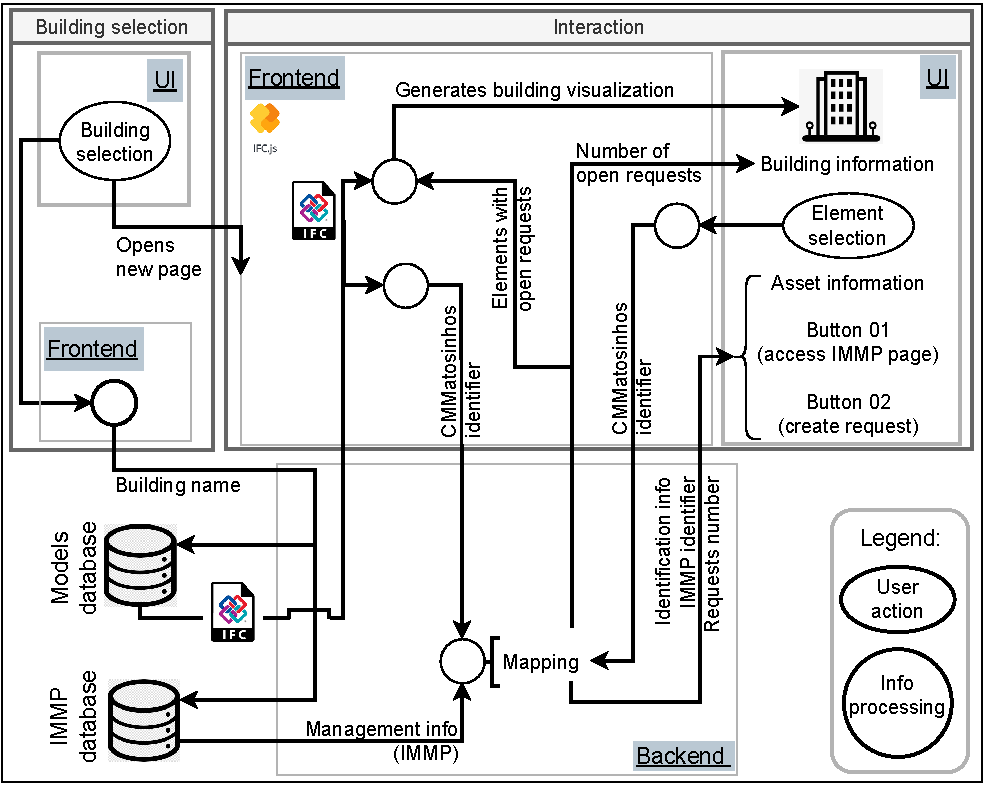
\includegraphics[width=0.48\textwidth]{Images/fluxo.pdf}
    \caption{Platform's information flow diagram}
    \label{fig_fluxo}
\end{figure}

Figure \ref{fig_plataforma} shows screenshots of the web platform from the perspective of a user of the manager type. Screenshot A shows the interaction page after the model is loaded with a 3D view of the entire building. When an asset is selected, the platform will appear as screenshot B. The page includes an upper section (screenshot C) with the building's identification and diverse options of visualization modes. The next section (screenshot D) warns about the presence and number of open requests. The side menu (screenshot E) displays information about the selected asset, and it appears on the user interface only when a piece of equipment or space is selected. In this menu, it is possible to visualize information identifying the asset and its number of open requests. In addition, two buttons allow the redirection to the asset's page within the IMMP and the creation of requests (screenshot F) associated with the asset. The request is registered within the IMMP platform, and the total number of open requests is updated automatically.

\begin{figure*}[!htb]
    \centering
    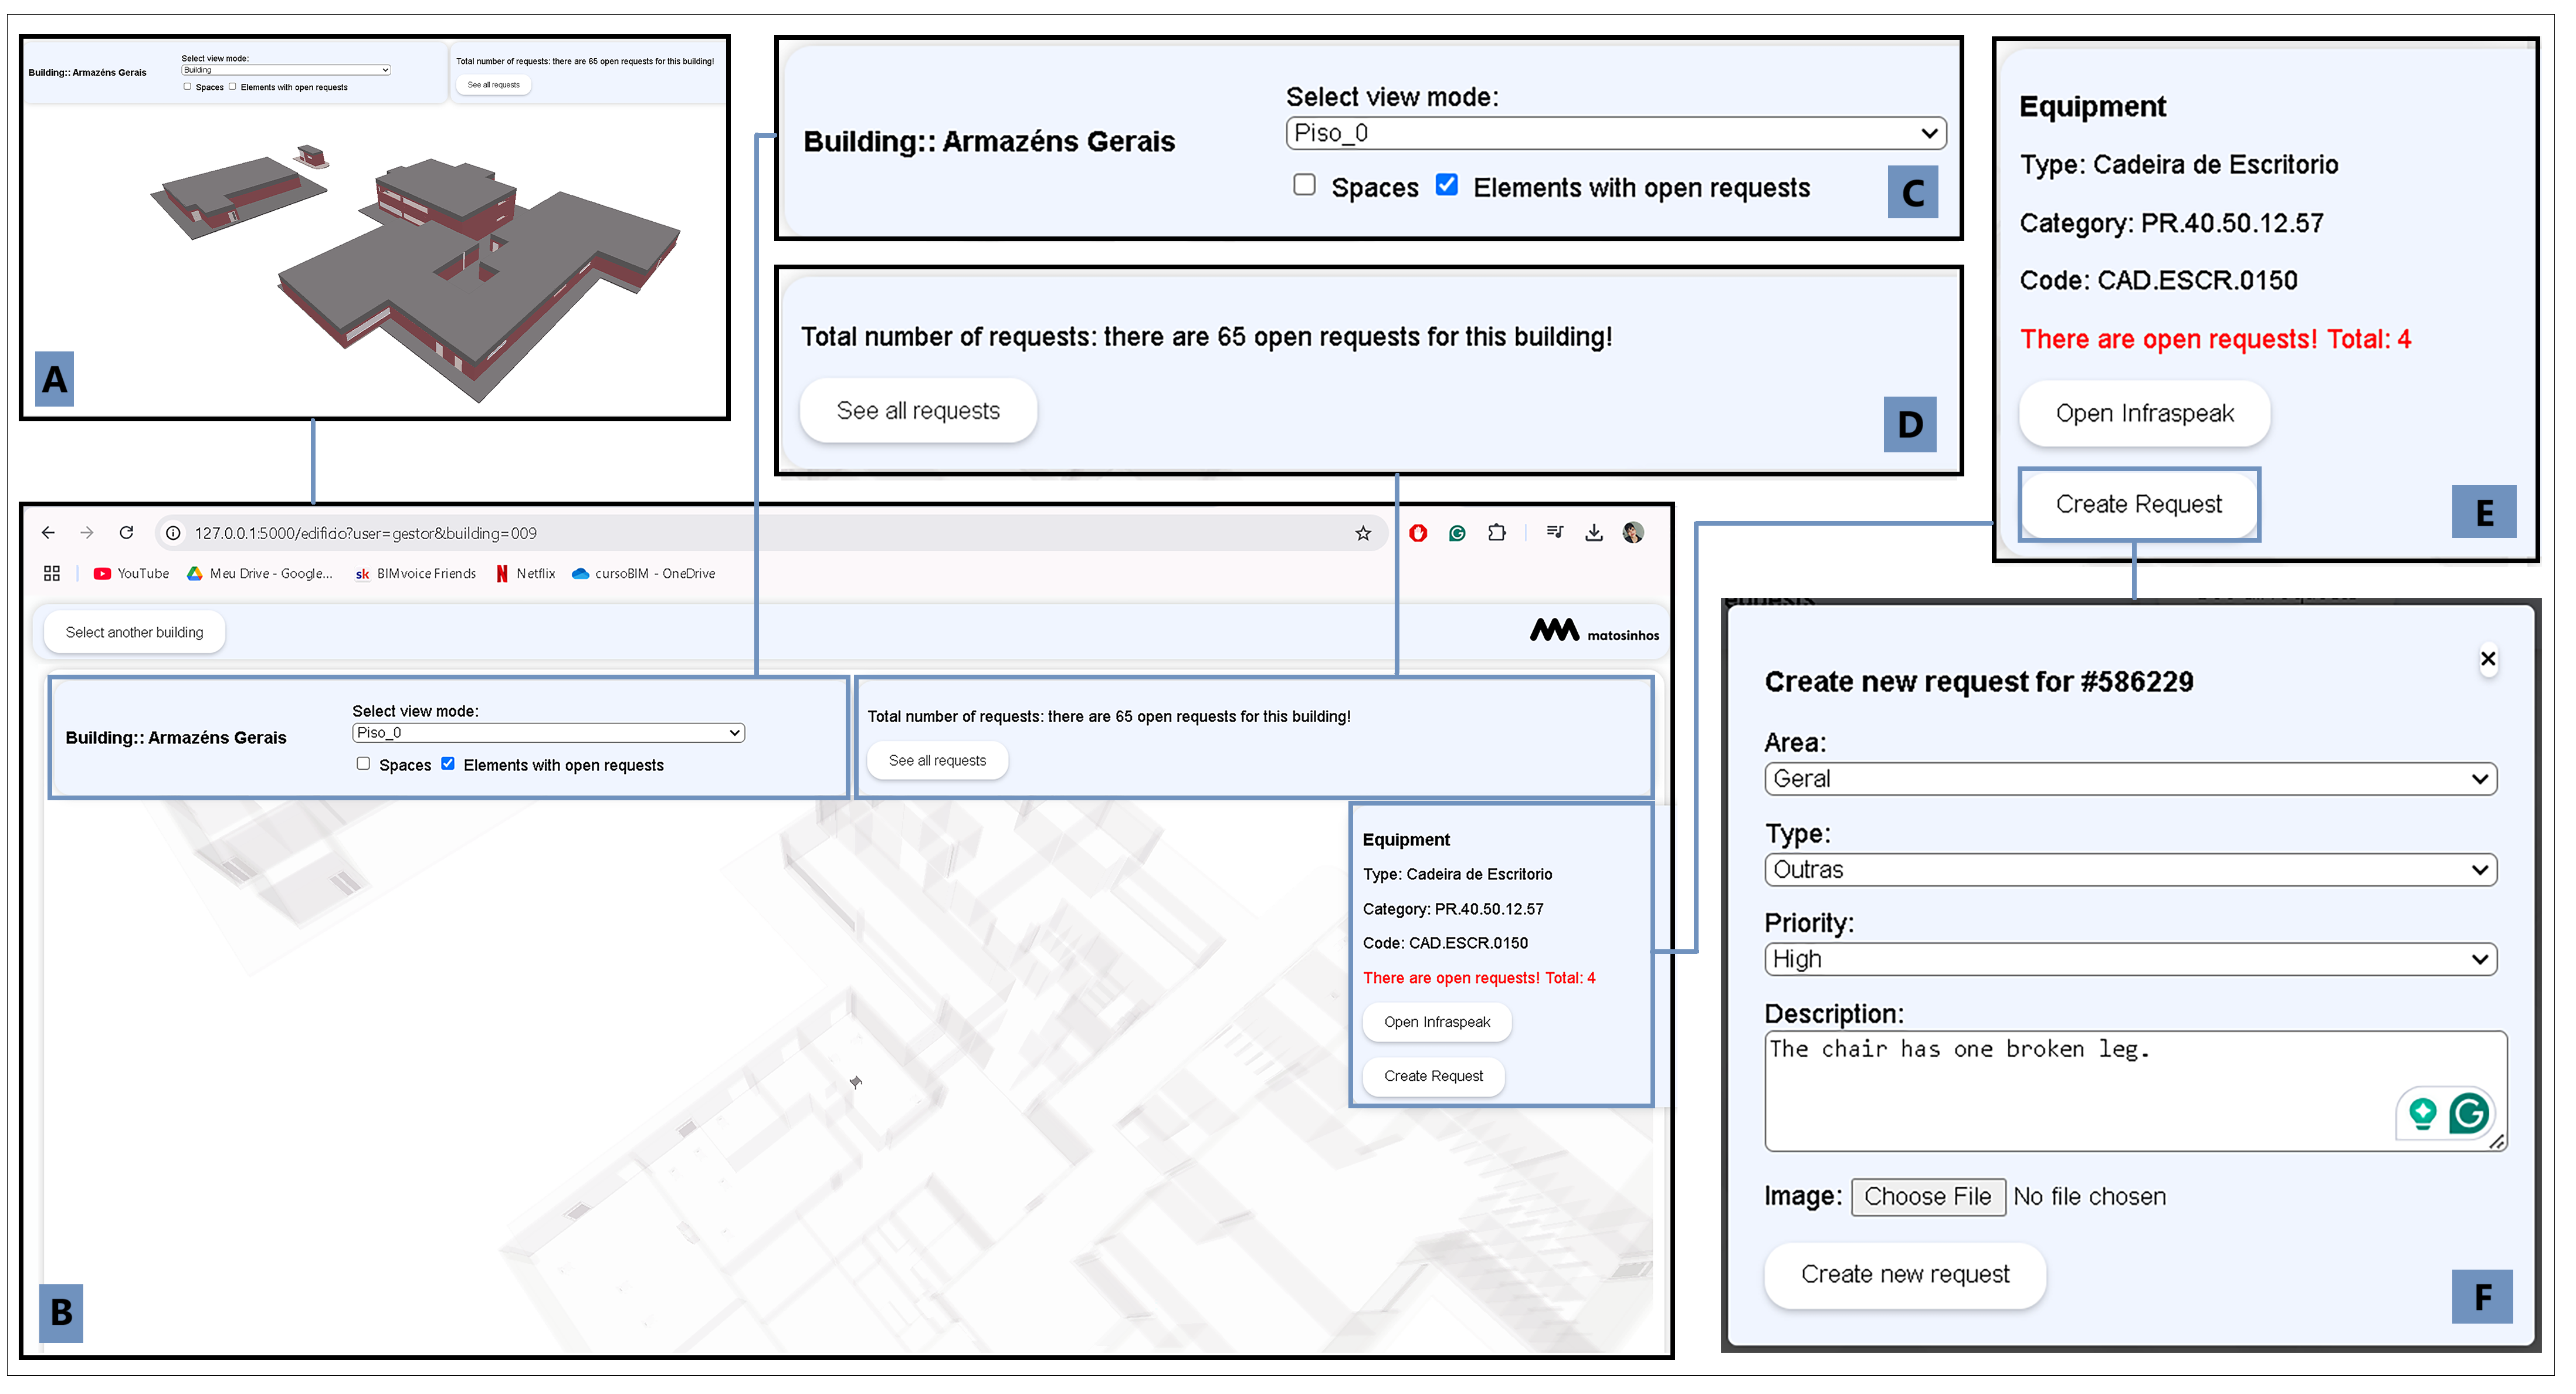
\includegraphics[width=0.87\textwidth]{Images/plataforma.png}
    \caption{Web platform}
    \label{fig_plataforma}
\end{figure*}

\section{Conclusion}
\label{sec:conclusion}

This work demonstrated the development and implementation of a BIM-based solution for FM, which has been integrated with an existing management platform that previously did not support BIM. The outcomes of this work provide a framework for future integration processes. This collaboration demonstrates that the operational sector does not need to completely alter its management system or adopt a different management platform to implement BIM effectively. However, it does need to prepare its inventory organization to facilitate digitalization. During the collaboration, an iterative process with CMMatosinhos helped to address the limitations encountered, showing that the close participation of managers is crucial for the FM sector's digitalization.

\section{Acknowledgements}
\label{sec:acknowledgements}

This work was partly financed by FCT / MCTES through national funds (PIDDAC) under the R\&D Unit Institute for Sustainability and Innovation in Structural Engineering (ISISE), under reference UIDB / 04029/2020 (doi.org/10.54499/UIDB/04029/2020), and under the Associate Laboratory Advanced Production and Intelligent Systems ARISE under reference LA/P/0112/2020. This work is also financed by national funds through FCT – Foundation for Science and Technology, under grant agreement PRT/BD/154416/2023 attributed to the 1st author, under the MIT Portugal Programme.

\bibliography{ISARC}

\end{document}
